\begin{minted}[]{r}
library(ggplot2)

# Side-note that if you run this as a file and not in the IDE the plots will
# actually be put into a PDF for you in the active working directory (here).

# We can use a randomly selected sample of the dataset for the graph.
# However, because the results should be reproducible, we should set an RNG seed.
set.seed(1000)

# Select the numbered rows of the numbers produced by sample.
# Sample picks 100 random numbers.
dsmall <- diamonds[sample(nrow(diamonds), 100),]
# The random comma at the end tells R that you're slecting ROWS, not columns.
# If you don't put this comma it assumes you're looking to select the columns.

qplot(log(carat), log(price), data = dsmall, geom = "smooth")
\end{minted}

\begin{minted}[]{text}
## `geom_smooth()` using method = 'loess' and formula = 'y ~ x'
\end{minted}

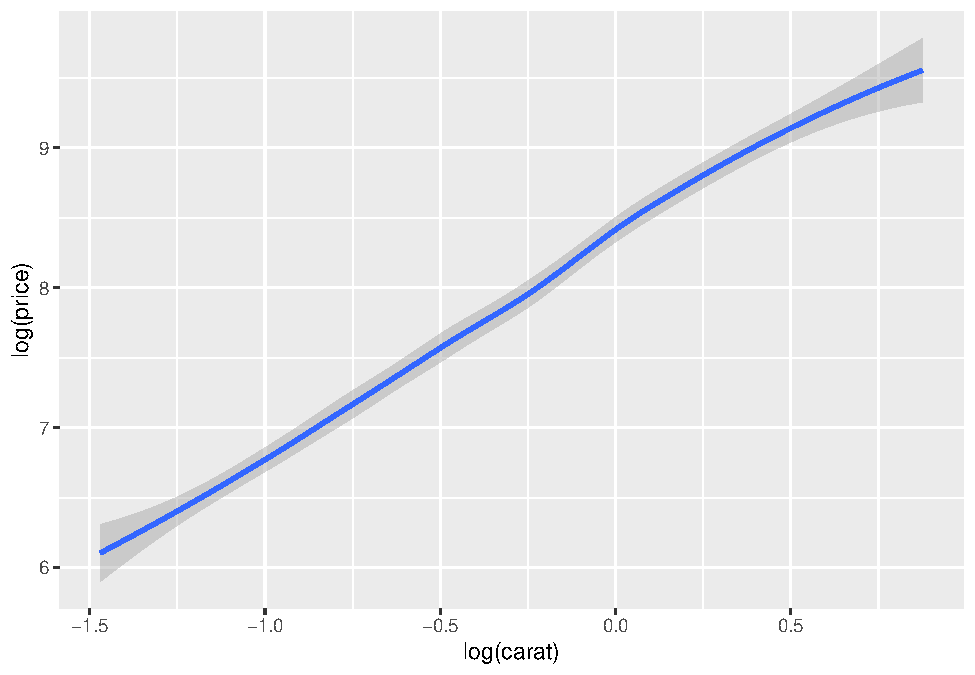
\includegraphics{C:/Users/Lewis/DataspellProjects/DataVis/Assignment/LaTeX/auxil/test2_files/figure-latex/unnamed-chunk-2-1.pdf}

\begin{minted}[]{r}
# Can supply multiple geoms in a vector
qplot(log(carat), log(price), data = dsmall, geom = c("point", "smooth"))
\end{minted}

\begin{minted}[]{text}
## `geom_smooth()` using method = 'loess' and formula = 'y ~ x'
\end{minted}

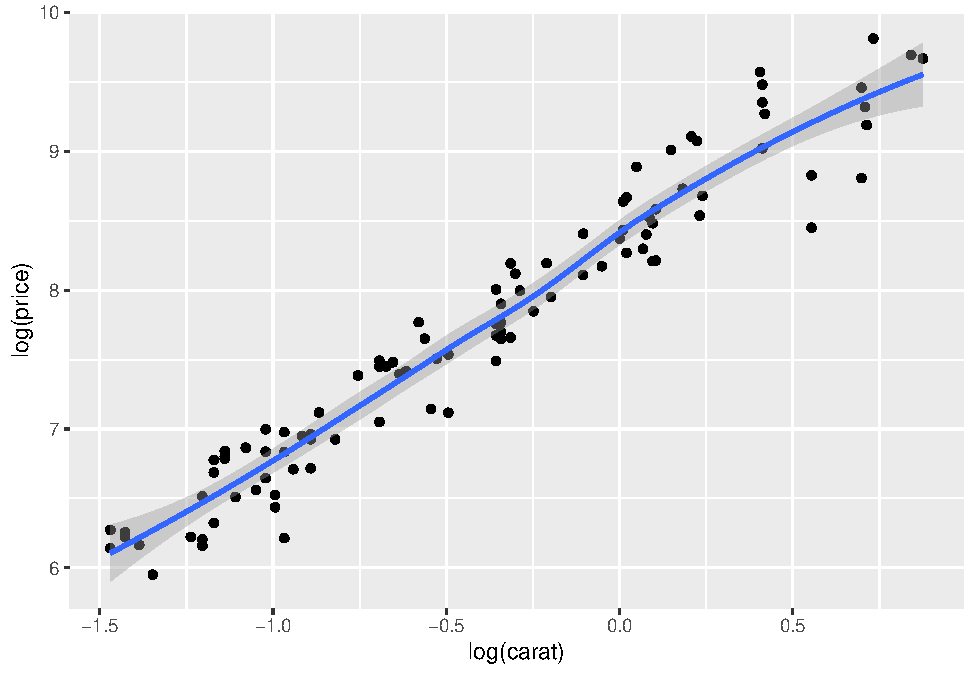
\includegraphics{C:/Users/Lewis/DataspellProjects/DataVis/Assignment/LaTeX/auxil/test2_files/figure-latex/unnamed-chunk-2-2.pdf}

\begin{minted}[]{r}
# Different smooth line?

# Span varies the smoothness of geom_smooth from 0 to 1 where 1 is the smoothest.
# It states that span is an unknown parameter, yet this does actually
# modify the produced graph. 0.2 is the minimum before R throws warnings.
# 0.1 works with warnings, but anything lower produces no smooth line.
# Though, using 0.1 means you might as well not even put a smooth line.
qplot(log(carat), log(price), data = dsmall, geom = c("point", "smooth"), span = 0.2)
\end{minted}

\begin{minted}[]{text}
## `geom_smooth()` using method = 'loess' and formula = 'y ~ x'
\end{minted}

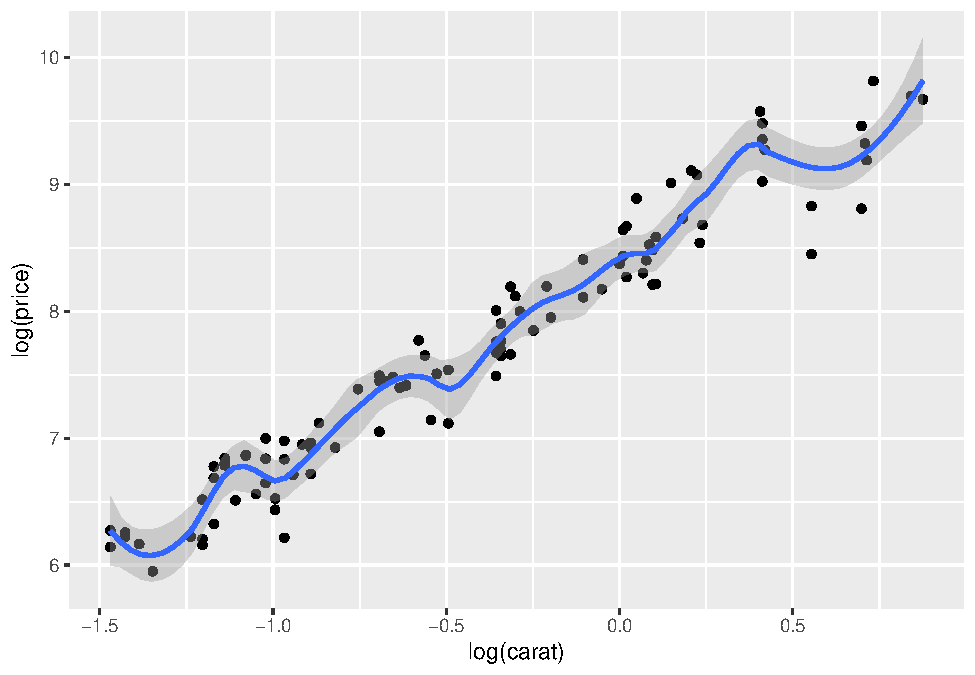
\includegraphics{C:/Users/Lewis/DataspellProjects/DataVis/Assignment/LaTeX/auxil/test2_files/figure-latex/unnamed-chunk-2-3.pdf}

\begin{minted}[]{r}
# You can also fit a linear model to the graph via lm.
qplot(log(carat), log(price), data = dsmall, geom = c("point", "smooth"), method = "lm")
\end{minted}

\begin{minted}[]{text}
## `geom_smooth()` using formula = 'y ~ x'
\end{minted}

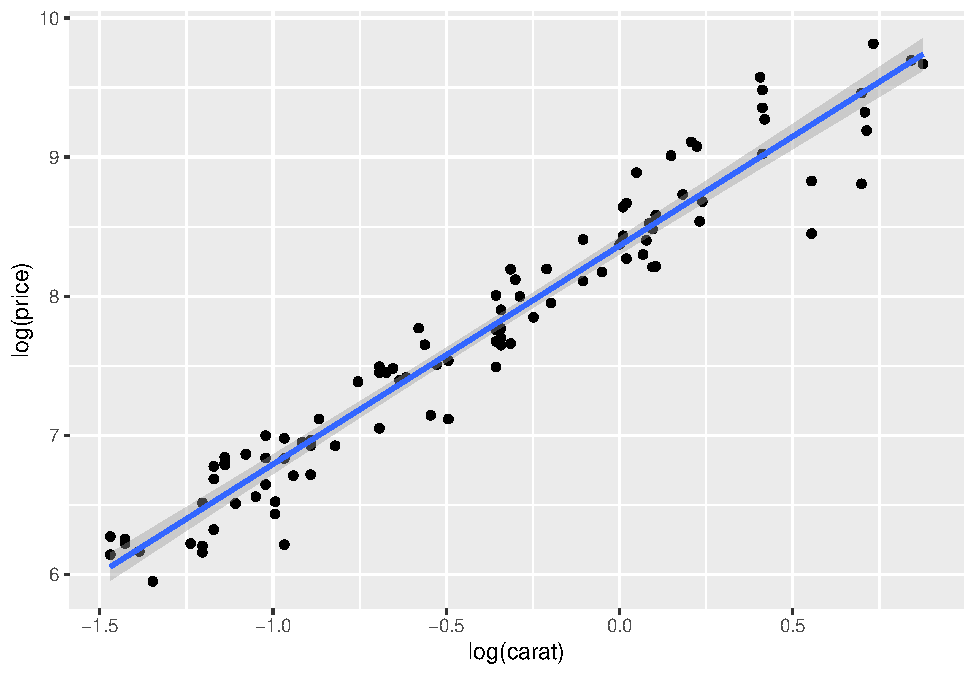
\includegraphics{C:/Users/Lewis/DataspellProjects/DataVis/Assignment/LaTeX/auxil/test2_files/figure-latex/unnamed-chunk-2-4.pdf}

\begin{minted}[]{r}
# Scatterplotting a different dataset, ggplot's builtin mpg (car fuel economy data)
qplot(displ, hwy, data = mpg, color = drv)
\end{minted}

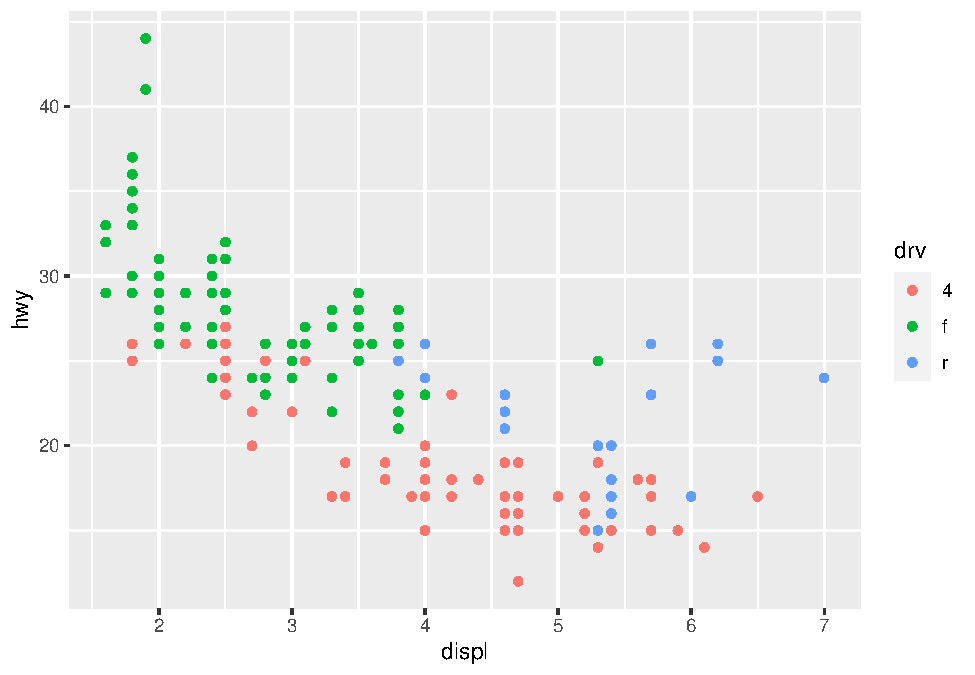
\includegraphics{C:/Users/Lewis/DataspellProjects/DataVis/Assignment/LaTeX/auxil/test2_files/figure-latex/unnamed-chunk-2-5.pdf}

\begin{minted}[]{r}
# If you provided a color argument to this, it would draw one smooth for every color.
qplot(displ, hwy, data = mpg, geom = c("point", "smooth"))
\end{minted}

\begin{minted}[]{text}
## `geom_smooth()` using method = 'loess' and formula = 'y ~ x'
\end{minted}

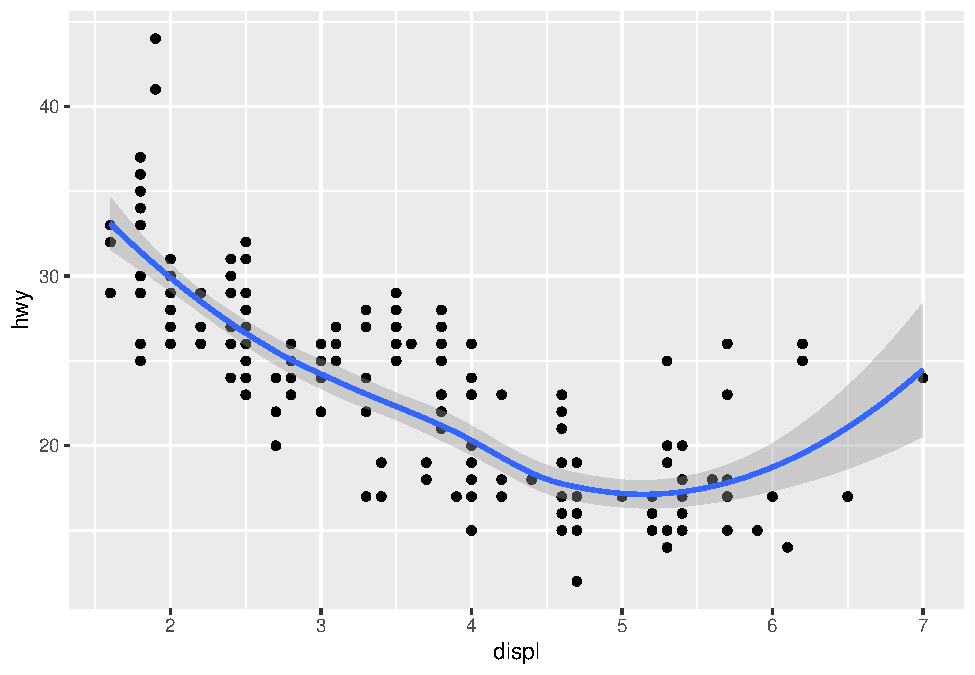
\includegraphics{C:/Users/Lewis/DataspellProjects/DataVis/Assignment/LaTeX/auxil/test2_files/figure-latex/unnamed-chunk-2-6.pdf}

\begin{minted}[]{r}
# Answers the question "How are engine size and fuel economy related?"
# Turning cylinder into a factor (categorical data).
# Basically counts the appearances of each value.
qplot(displ, hwy, data = mpg, color = factor(cyl))
\end{minted}

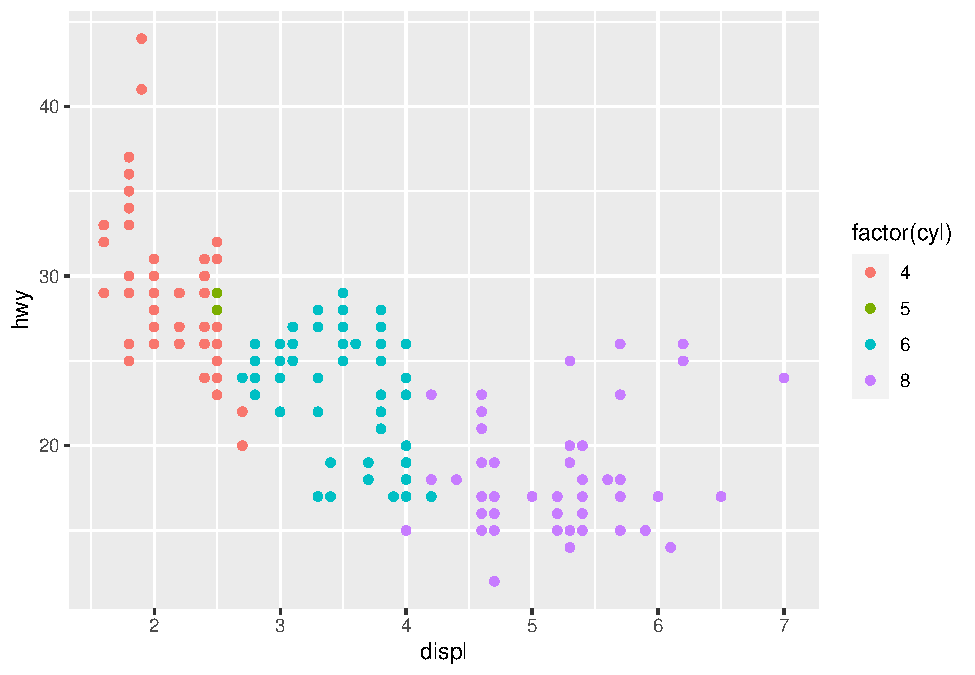
\includegraphics{C:/Users/Lewis/DataspellProjects/DataVis/Assignment/LaTeX/auxil/test2_files/figure-latex/unnamed-chunk-2-7.pdf}

\begin{minted}[]{r}
# We can use all arguments previously shown at once.
# Note that there aren't enough 5 cylinders to fit a line, so there isn't one.
qplot(displ, hwy, data = mpg, color = factor(cyl),
      geom = c("point", "smooth"), method = "lm")
\end{minted}

\begin{minted}[]{text}
## `geom_smooth()` using formula = 'y ~ x'
\end{minted}

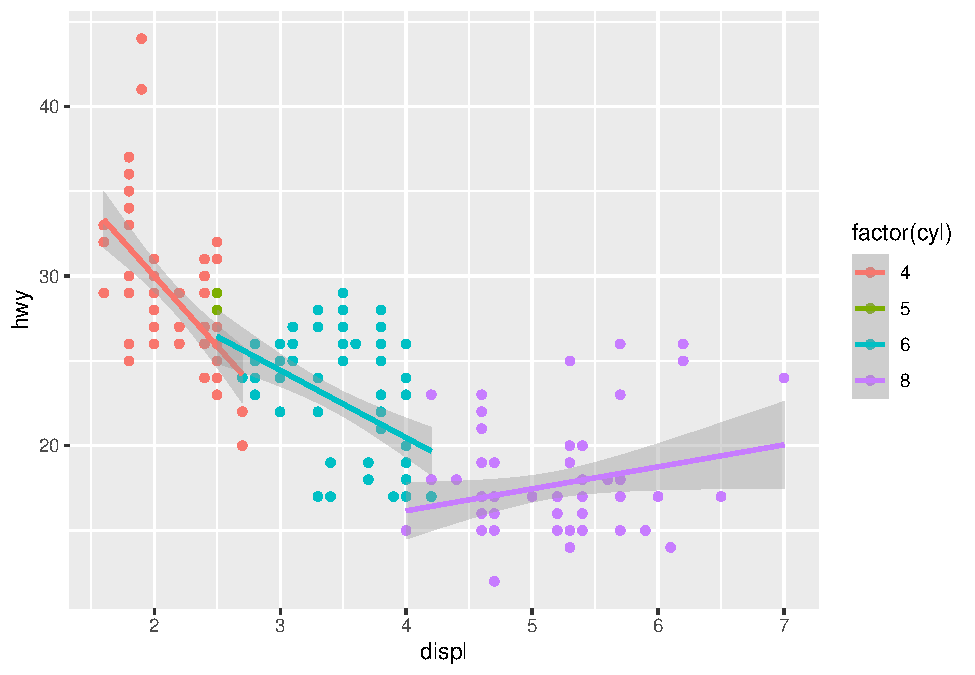
\includegraphics{C:/Users/Lewis/DataspellProjects/DataVis/Assignment/LaTeX/auxil/test2_files/figure-latex/unnamed-chunk-2-8.pdf}

\begin{minted}[]{r}
### --- Faceting --- ###


# . acts as a placeholder, indicating that there's no variable.
# Results in three seperate histograms, one of each drive class.
qplot(hwy, data = mpg, facets = drv ~ ., binwidth = 2)
\end{minted}

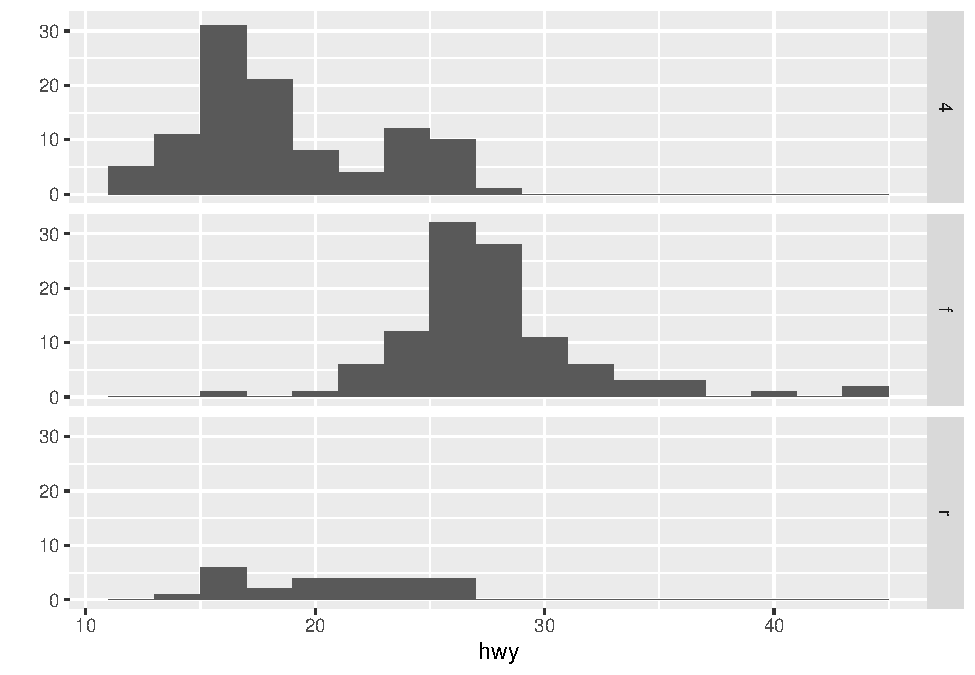
\includegraphics{C:/Users/Lewis/DataspellProjects/DataVis/Assignment/LaTeX/auxil/test2_files/figure-latex/unnamed-chunk-2-9.pdf}

\begin{minted}[]{r}
# Could add colors. Doesn't help much though.

# Flips sideways. displ is displacement. Air movement per engine rev possibly
qplot(displ, hwy, data = mpg, facets = . ~ drv, geom = c("point", "smooth"))
\end{minted}

\begin{minted}[]{text}
## `geom_smooth()` using method = 'loess' and formula = 'y ~ x'
\end{minted}

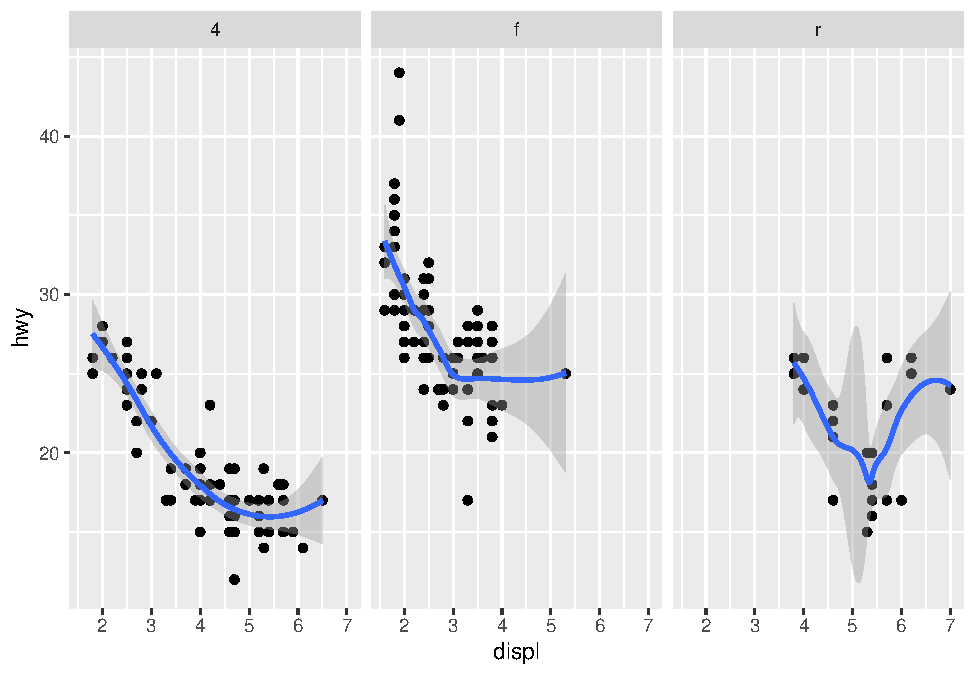
\includegraphics{C:/Users/Lewis/DataspellProjects/DataVis/Assignment/LaTeX/auxil/test2_files/figure-latex/unnamed-chunk-2-10.pdf}

\begin{minted}[]{r}
# Reusing the diamond set.
qplot(carat, data = diamonds, facets = color ~ ., geom = "histogram")
\end{minted}

\begin{minted}[]{text}
## `stat_bin()` using `bins = 30`. Pick better value with `binwidth`.
\end{minted}

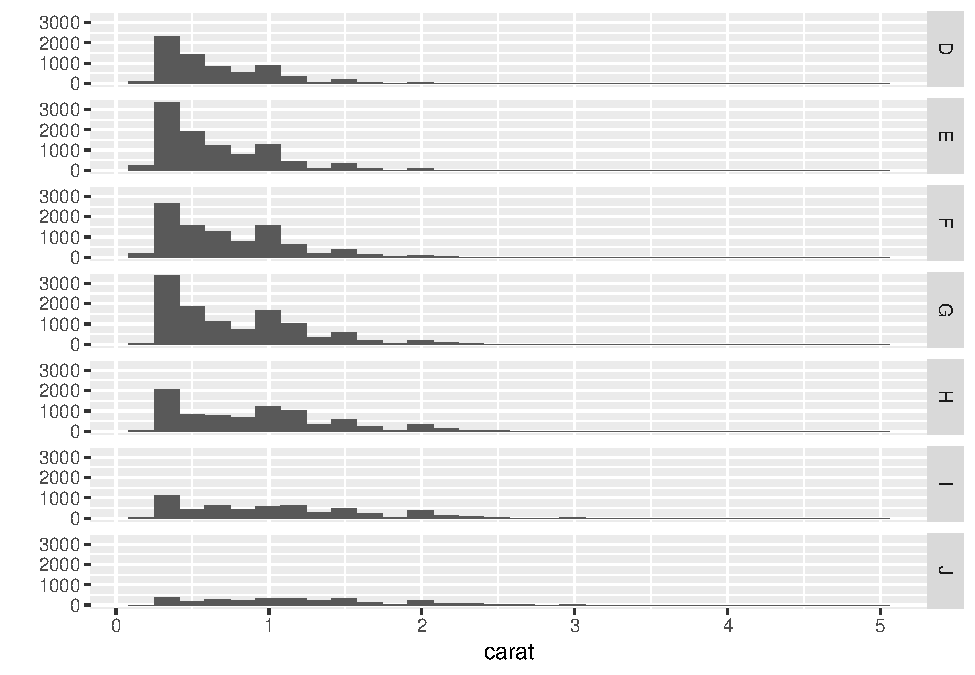
\includegraphics{C:/Users/Lewis/DataspellProjects/DataVis/Assignment/LaTeX/auxil/test2_files/figure-latex/unnamed-chunk-2-11.pdf}

\begin{minted}[]{r}
# ..density.. tells ggplot to map the density as the Y-axis, instead of just counting.
qplot(carat, ..density.., data = diamonds, facets = color ~ ., geom = "histogram")
\end{minted}

\begin{minted}[]{text}
## `stat_bin()` using `bins = 30`. Pick better value with `binwidth`.
\end{minted}

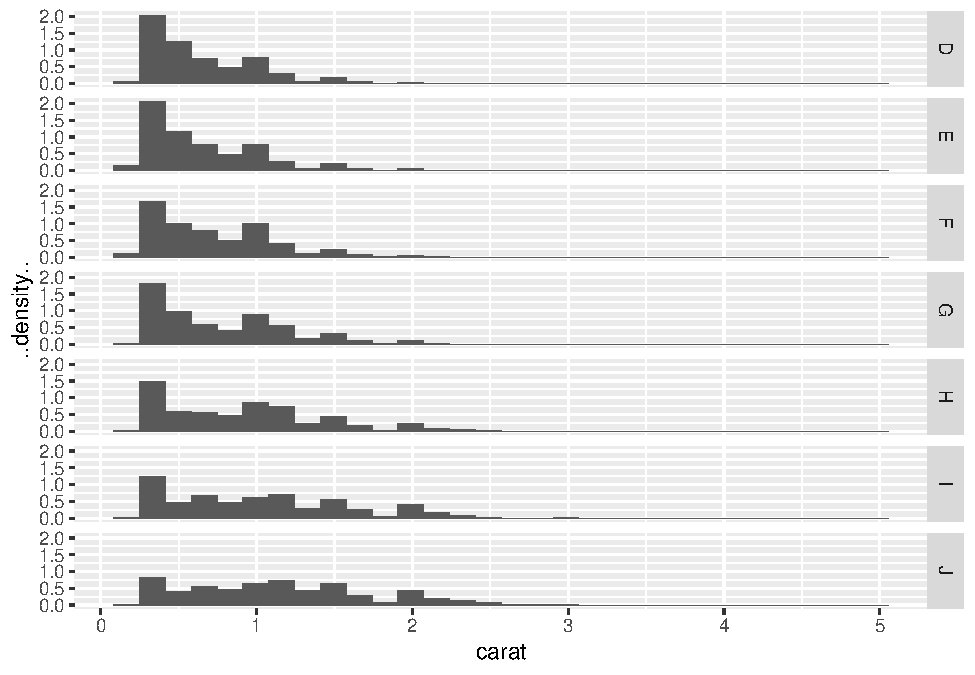
\includegraphics{C:/Users/Lewis/DataspellProjects/DataVis/Assignment/LaTeX/auxil/test2_files/figure-latex/unnamed-chunk-2-12.pdf}

\begin{minted}[]{r}
# Plots thirty five histograms by also grouping by cut.
qplot(carat, data = diamonds, facets = color ~ cut, geom = "histogram")
\end{minted}

\begin{minted}[]{text}
## `stat_bin()` using `bins = 30`. Pick better value with `binwidth`.
\end{minted}

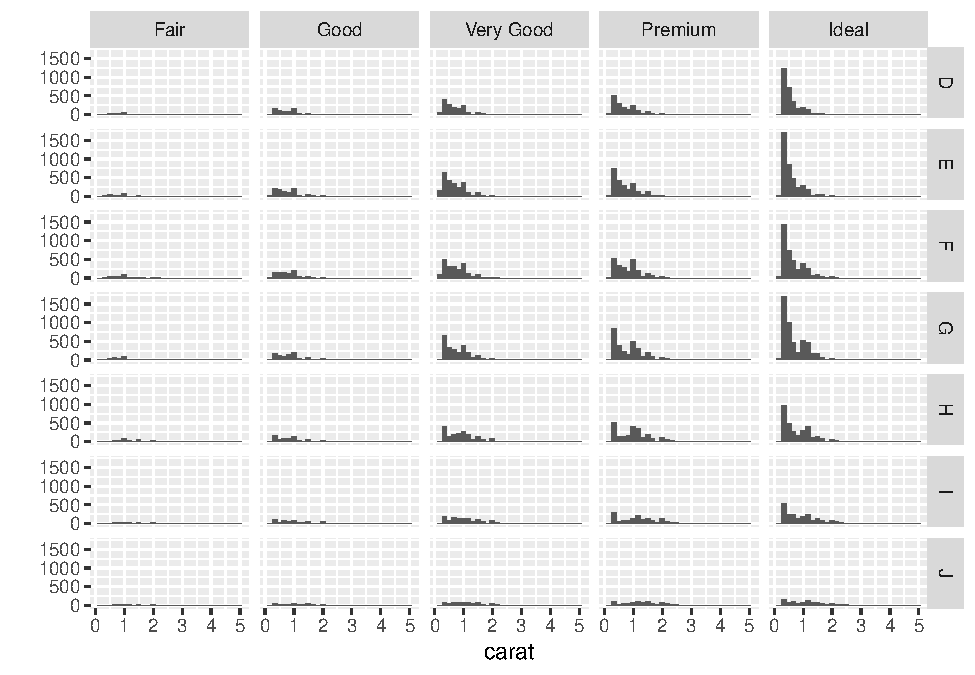
\includegraphics{C:/Users/Lewis/DataspellProjects/DataVis/Assignment/LaTeX/auxil/test2_files/figure-latex/unnamed-chunk-2-13.pdf}
